\chapter{Fundamentação teórica}\label{chapter-fundamentacao}

% \begin{KeepFromToc}
% \end{KeepFromToc}

\chapterprecis{Este capítulo aprensenta uma introdução sobre as arquiteturas monolítica e de microsserviços}\index{sinopse de capítulo}

Assim como este capítulo, a maioria dos engenheiros de \emph{software} fala da arquitetura de microsserviços contrastando-a com a arquitetura monolítica, pois essa última é a abordagem mais comumente usada de arquitetura de \emph{software}. Porém, é importante ter em mente que existem outros tipos de arquitetura que não se encaixam nem como de microsserviços nem como monolíticas, tal como as arquiteturas cliente-servidor e orientada a serviços \cite{martin-fowler-microservice-tradeoffs}.
% https://www.alura.com.br/artigos/padroes-arquiteturais-arquitetura-software-descomplicada
% arquitetura hexagonal parece interessante

\section{As aplicações monolíticas}\label{sessao-monolitos}

Aplicações monolíticas, também chamadas de monólitos, são aplicações que possuem as camadas de acesso aos dados, de regras de negócios e de interface de usuário em um único programa em uma única plataforma. As aplicações monolíticas são autocontidas, totalmente independentes de outras aplicações e são feitas não para uma tarefa em particular, mas sim para serem responsáveis por todo o processo para completar determinada função, assim tendo pouca ou nenhuma modularidade. Elas podem ser organizadas das mais variadas formas e fazer uso de padrões arquiteturais, mas são limitadas em muitos outros aspectos, apresentados na \autoref{subsection-monolitos-limitacoes} \cite{wiki_monolithic_2022}.

\subsection{Benefícios}

O maior e melhor benefício da arquitetura monolítica é sua simplicidade. Os monólitos são simples para desenvolver, para implantar, e para escalar, ademais uma aplicação simples é uma aplicação mais fácilmente entendida pelos seus desenvolvedores, fato que por sí só já melhora sua manutenibilidade. Porém, vale ressaltar que simplicidade não necessariamente implica em facilidade.

Outra vantagem dos monólitos é a facilidade de desenvolvimento da sua infraestrutura. Por não possuirem dependências com outras aplicações e nem precisarem se dedicar a comunicação externa, os monólitos têm uma infraestrutura fácil de elaborar.
%e além disso, neles geralmente não é necessário haver comunicação entre diferentes serviços ou máquinas, então os desenvolvedores não precisarão se preocupar com a complexidade que acompanha essa comunicação.

Entretanto, esses benefícios só são válidos até certo ponto. Depois que uma aplicação monolítica ou o time que a desenvolve cresce muito, ela pode se tornar um emaranhado complexo de funcionalidades que são difíceis de diferenciar, de separar e de manter, e os problemas dos monólitos começam a ficar evidentes \cite{microservicesIO_monolithic_architecture}.

\subsection{Limitações}\label{subsection-monolitos-limitacoes}

\subsubsection{Crescimento, velocidade de desenvolvimento, e manutenção}
% subsubsection tamanho da aplicação
Quando aplicações monolíticas chegam a certo tamanho, pode se tornar muito difícil desenvolver funcionalidades novas, ou mesmo prover manutenção às já existentes, devido a diversos problemas que começam a surgir, tais como: lentidão da IDE por conta do tamanho do código, prejudicando a produtividade dos desenvolvedores; sobrecarregamento do contêiner ou máquina que hospeda a aplicação, aumentando o tempo de início; e dificuldade de entendimento da aplicação e de realizar alterações nela, diminuindo a velocidade de desenvolvimento e a qualidade do código. Padrões de organização podem amenizar a situação, mas não eliminam o problema \cite{microservicesIO_monolithic_architecture}.

\subsubsection{Escalabilidade}
O escalamento de aplicações monolíticas também pode se tornar um problema, pois ele só pode ser feito em uma dimensão. É possível escalar o volume de operações executando mais cópias de um monólito, mas não é possível fazer isso com o volume dos dados, pois cada cópia precisará acessar todos os dados, o que aumenta o consumo de memória e o tráfego de entradas e saídas (\emph{I/O}). Também não é possível escalar os componentes independentemente, não permitindo ajustar poder de processamento ou memória quando ou onde adequado \cite{microservicesIO_monolithic_architecture}.

% Scaling the application can be difficult - a monolithic architecture is that it can only scale in one dimension. On the one hand, it can scale with an increasing transaction volume by running more copies of the application. Some clouds can even adjust the number of instances dynamically based on load. But on the other hand, this architecture can’t scale with an increasing data volume. Each copy of application instance will access all of the data, which makes caching less effective and increases memory consumption and I/O traffic. Also, different application components have different resource requirements - one might be CPU intensive while another might memory intensive. With a monolithic architecture we cannot scale each component independently. \cite{microservicesIO_monolithic_architecture}

\subsubsection{Reutilização}
O alto acoplamento entre as partes de aplicações monolíticas dificulta a reutilização delas, o que pode causar esforço e código repetidos.

\subsubsection{Implantação}
Realizar alterações em qualquer componente de um monólito implica na necessidade de reimplantar toda a aplicação, mesmo as partes que não têm ligação com as alterações, o que aumenta riscos associados a falhas na implantação e consequentemente desencoraja a prática de implantação contínua \cite{microservicesIO_monolithic_architecture}.

\subsubsection{Confiabilidade e resiliência}
O alto acoplamento existente entre as partes da aplicação monolítica permite que falhas relativamente pequenas possam prejudicar toda a aplicação, inclusive as partes que não tiveram relação com a falha.

\subsubsection{Flexibilidade de tecnologias}
As escolhas de tecnologias para novas funcionalidades são mais limitadas - um projeto tende a usar apenas um certo grupo de tecnologias porque realizar \emph{upgrades} ou mudanças de tecnologias é uma tarefa complexa e pode causar problemas de compatibilidade \cite{microservicesIO_monolithic_architecture}.

\subsubsection{Divisão de times}
Quando um monólito alcança determinado tamanho, é desejável dividir os desenvolvedores em times que têm foco em partes funcionais ou do domínio específicas da aplicação. Entretanto, ter times separados no desenvolvimento de uma mesma aplicação monolítica é mais difícil e menos proveitoso, porque nunca serão totalmente independentes, visto que precisam coordenar o desenvolvimento e as implantações da aplicação \cite{microservicesIO_monolithic_architecture}.

% ---
\section{Os microsserviços}
% ---

Microsserviços é uma abordagem de arquitetura de \emph{software}. Aplicações com uma arquitetura de microsserviços são separadas em partes, chamadas de microsserviços, que são classificadas em tipos (apresentados na \autoref{fundamentacao-tipos-microsservicos}) e se comunicam por meio de uma rede. Microsserviços oferecem capacidades de negócio (funcionalidades relacionadas às regras de negócio da aplicação) ou capacidades de plataforma (funcionalidades relacionadas ao ambiente de execução da aplicação), tratando um aspecto em particular da aplicação. Eles se comunicam por meio de APIs bem definidas, contratos de dados e configurações. O “micro” em microsserviços faz referência não ao tamanho do serviço, mas sim ao seu escopo de funcionalidade, pois trata-se de oferecer apenas uma determinada funcionalidade, tornando-se especialistas nela. Assim sendo, microsserviços não necessariamente devem ser pequenos em tamanho, mas fazem apenas uma tarefa e a fazem bem \cite{Familiar2015,livro-building-microservices}.
 
Sendo especialistas em apenas uma tarefa, microsserviços têm características e comportamentos que os diferenciam de outras arquiteturas orientadas a serviços, os quais serão discutidos no \autoref{chapter-caracteristicas}.

A \autoref{figura_arquitetura_microsservicos} exemplifica uma aplicação com arquitetura de microserviços. Inicialmente os usuários da aplicação (camada \emph{Clients}) fazem requisições à API para obter as informações desejadas. O \hyperref[boas-praticas-api-gateway]{\emph{API Gateway}} é reponsável por gerenciar as chamadas aos microsserviços e fará as devidas requisições para os devidos microsserviços (localizados na camada \emph{Container Orchestration}). Esses microsserviços, então, executarão a lógica apropriada de acordo com a requisição recebida, possivelmente usando informações registradas no banco de dados apropriado (camada \emph{Data Store}).

\begin{figure}[htb]
	\caption{\label{figura_arquitetura_microsservicos}Exemplo de aplicação com arquitetura de microsserviços}
	\begin{center}
	    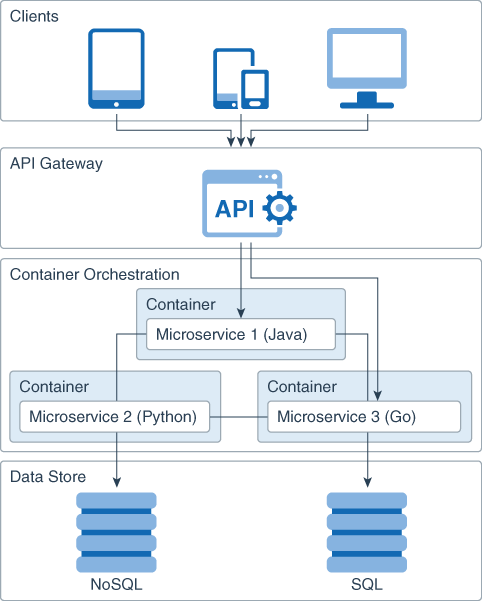
\includegraphics[scale=0.8]{Imagens/microservice_architecture.png}
	\end{center}
	\legend{Fonte: \citeonline{oracle_microservices}}
\end{figure}

% A ilustração mostra as camadas da arquitetura de microsserviços. A primeira camada é a camada do cliente, que contém: os computadores, laptops e dispositivos móveis. A segunda camada é a camada do gateway de API, que redireciona as solicitações do cliente para os microsserviços apropriados. A terceira camada é a camada de orquestração de contêineres, com todos os microsserviços agrupados dentro de uma orquestração de contêineres. Cada um dos microsserviços está em contêiner. Eles se comunicam com os clientes por meio do gateway de API. A quarta camada é a camada de armazenamento de dados. Cada um dos microsserviços em contêiner que implementam persistência se comunica a apenas um armazenamento de dados. Os armazenamentos de dados exibidos são NoSQL e SQL.


% Microsserviços são uma abordagem arquitetônica e organizacional do desenvolvimento de software na qual o software consiste em pequenos serviços independentes que se comunicam usando APIs bem definidas. Esses serviços pertecem a pequenas equipes autossuficientes.

% A arquitetura de microsserviços (AMS) está ganhando força no desenvolvimento e entrega de aplicações de software como um conjunto de pequenos serviços granulares que podem ser integrados por meio de mecanismos de comunicação leve, normalmente APIs RESTful [10]. Microsserviços são componentes pequenos e facilmente entendíveis que possuem capacidades de negócio no meio dos serviços [11]. Esses serviços podem ser escalados independentemente (já que são desacoplados) pela implementação de \texttt{stacks} de tecnologias diferentes [2]. Muitos pesquisadores e praticantes dizem que AMS é uma evolução da Arquitetura orientada a serviços (AOS), como visto no contexto de serviços independentes/auto-suficientes e de natureza leve [12]. Por outro lado, AMS pode ser diferenciada da AOS em termos de compartilhamento de componentes, comunicação de serviços, mediação de serviços, e acesso remoto aos serviços [13]. (Bar, f., 2018, tradução nossa). \cite{WASEEM2020110798}
% % AOS é construida com base na ideia de compartilhar o máximo possível, enquanto AMS, o mínimo possível [13, 14]. AMS usa um estilo coreografico para comunicação inter-serviços, enquanto AOS aplica um estilo de orquestração para coordenação de serviços. Para mediação de serviços, AMS usa a camada de API que atua como uma fachada para o serviço, enquanto AOS adota o conceito de um \texttt{middleware} mensageiro para coodenação de serviços. Além disso, AMS em grande parte depende do protocolo REST e mensageria simples como protocolo de acesso remoto ao serviço; entretanto, AOS consegue lidar com diferentes tipos de protocolo de acesso remoto, incluindo mensageria simples para acessar serviços remotos [13].

\subsection{Tipos de microsserviços}\label{fundamentacao-tipos-microsservicos}

\subsubsection{Serviço de dados (\emph{data service})}
Tipo de serviço de mais baixo-nível. É responsável por receber e tratar dados, assim fornecendo acesso a determinado domínio e suas regras. Quando um serviço de dados realiza apenas operações relacionadas a um determinado domínio da aplicação, ele também é chamado de serviço de domínio.

\subsubsection{Serviço de negócio (\emph{business service})}
Em determinados momentos as operações precisam de mais de um modelo do domínio para serem representadas em um serviço. Assim, os serviços de negócio agregam dados e oferecem operações mais complexas. Eles englobam vários serviços de domínio e proveem uma funcionalidade do negócio de nível mais alto, podendo também encapsular domínios relacionados. Por exemplo, em um site de cursos \emph{online}, um serviço de negócio poderia prover uma funcionalidade chamada "Matricular Aluno", que envolveria as operações de inserir aluno no serviço de cursos, inserir aluno no serviço de pagamento, e inserir aluno no serviço de gamificação.

\subsubsection{Serviço de tradução (\emph{translation service})}
Um serviço de tradução é um intermediário entre a aplicação e um recurso externo, provendo uma forma de acessar esse recurso. No caso desse serviço externo sofrer mudanças, pode-se realizar as alterações consequentemente necessárias em apenas um lugar, nesse serviço de tradução. Por exemplo, a aplicação pode consumir uma API externa por meio do serviço de tradução, pedindo para que ele faça uma requisição para essa API, e então recebendo a resposta. % App --> translation service --> Api externa

\subsubsection{Serviço de ponta (\emph{edge service})}
É um serviço que serve diretamente ao cliente, sendo customizado para atender necessidades específicas desse cliente. Por exemplo, pode existir um serviço de ponta para clientes móveis e outro serviço de ponta para clientes web.

\subsubsection{Serviço agregador (\emph{aggregator service})}
Esse tipo de serviço consolida ou agrega dados de vários serviços em uma única requisição ou resposta, simplificando as interações com o cliente e reduzindo o número de chamadas necessárias por meio da rede. 
% Em vez de exigir que o cliente orquestre várias chamadas para diferentes microsserviços, um serviço agregador atua como um intermediário que busca dados de várias fontes, os processa e retorna um resultado unificado.
